% 2023年北京高考数学第9题：庑殿顶几何结构
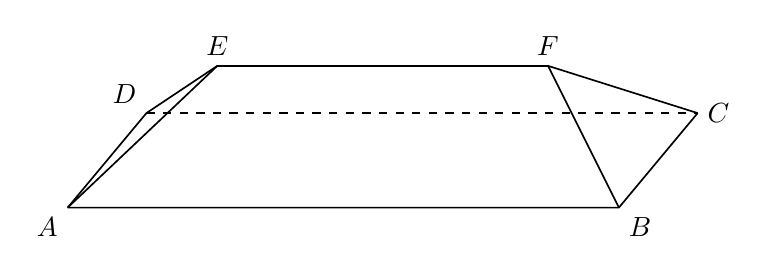
\begin{tikzpicture}[>=stealth,line width=0.6pt,font=\normalsize]
  \coordinate (A) at (0,0);
  \coordinate (B) at (7.0,0);
  \coordinate (C) at (8.0,1.2);
  \coordinate (D) at (1.0,1.2);
  \coordinate (E) at (1.9,1.8);
  \coordinate (F) at (6.1,1.8);

  % 实线可见边
  \draw (A) -- (B) -- (C);
  \draw (A) -- (D);
  \draw (E) -- (F);
  \draw (E) -- (A);
  \draw (E) -- (D);
  \draw (F) -- (B);
  \draw (F) -- (C);

  % 虚线不可见底边
  \draw[dashed] (D) -- (C);

  % 顶点标注
  \node[below left] at (A) {$A$};
  \node[below right] at (B) {$B$};
  \node[right] at (C) {$C$};
  \node[above left] at (D) {$D$};
  \node[above] at (E) {$E$};
  \node[above] at (F) {$F$};
\end{tikzpicture}
